\documentclass[a4paper,10pt]{article}

\usepackage[margin=2cm]{geometry}
\usepackage{graphicx}
\usepackage{hyperref}
\usepackage[all]{hypcap}
\usepackage{tabu}
\usepackage[title,titletoc,toc]{appendix}
\usepackage[english]{babel}
\usepackage{fontspec}
\usepackage[style=authoryear,backend=biber,sorting=nyt,dashed=false,urldate=long,abbreviate=false]{biblatex}
\usepackage{float}
\usepackage{fancyhdr}
\usepackage{microtype}

\addbibresource{references.bib}

\setlength{\headheight}{15.2pt}
\pagestyle{fancy}
\lhead{}
\chead{}
\rhead{\bfseries Software Requirements Specification}
\lfoot{Team Echo}
\cfoot{COS301 Software Engineering}
\rfoot{Page \thepage}
\renewcommand{\headrulewidth}{0.4pt}
\renewcommand{\footrulewidth}{0.4pt}

\setlength{\parindent}{0pt}
\setlength{\parskip}{1ex plus 0.5ex minus 0.2ex}

\frenchspacing

\title{
\includegraphics[width=12cm]{Eeufeeslogo.jpg} \\
       Software Requirements Specification \\ 
       and \\
       Technology Neutral Process Design \\
       Research Paper Management System \\
       \vspace{0.5cm}
       University of Pretoria \\
       \vspace{1.0cm}
       }

\date{} 
\author{Team Echo\\
	\vspace{0.5cm} \\
	\begin{tabu} to \textwidth { X[l] X[l]}
		\hline
		\textbf{Surname, First Name (Initial)}	& \textbf{Student Number}	\\ \hline \hline
		Bode, Elizabeth (EF)			& 14310156		\\ \hline
		Bondjobo, Jocelyn (JM)		& 13232852		\\ \hline
		Broekman, Andrew (A)		& 11089777		\\ \hline
		Loreggian, Fabio (FR)			& 14040426		\\ \hline
		Schutte, Gerome (GC)		& 12031519		\\ \hline
		Sefako, Motsitsiripe (MG)		& 12231097		\\ \hline
		Singh, Emilio (E)			& 14006512		\\ \hline
		\hline
	\end{tabu}}

\DefineBibliographyStrings{english}{%
urlseen = {\mbox{Accessed} on},
urlfrom = {[Online]},
in = {In},
}
\DeclareFieldFormat{url}{\bibstring{urlfrom}\space\url{#1}}
\DeclareFieldFormat{urldate}{\addcomma\space[\bibstring{urlseen}\space#1]}
\addto\captionsenglish{
  \renewcommand{\contentsname}
    {Table of Contents}
}

\begin{document}
\maketitle
\thispagestyle{empty}
\clearpage

\newpage
\pagenumbering{roman}
\thispagestyle{empty}
\tableofcontents
\clearpage

\newpage
\pagenumbering{arabic}

\section{Vision}
The client, Vreda Pieterse, from the University of Pretoria has requested a system to keep track of research publications in the Department of Computer Science at the University of Pretoria. The scope of the system is managing the administration involved in tracking of research publications within the department. However collaboration on research papers is outside of the scope as a version control system is in use currently. The system is required to keep track of all publications and the associated meta data around the publications.

The department currently consists of various research groups, with various contributors, all producing research publications which should be tracked. As the University of Pretoria is rewarded for research produced, it is important for both the heads of research groups and the Head of Department to monitor the progress of current publications, and to gather other metrics to assist in other departmental planning.

The most important requirements as set out by the client are:
\begin{enumerate}
\item Monitoring the research output by the department through metrics by the Head of Department and heads of the research groups
\item Tracking the status of research publications
\item Being able to produce customized reports based on user defined values
\end{enumerate}

\section{Background}
This project was commissioned based on the following three problems faced by the client
\begin{itemize}
\item Limitations of current system:
	\begin{itemize}
	\item The current system used by the client involves utilizing one common Microsoft Excel spreadsheet document to keep track of the status of current research publications. A problem with this solution is that it causes data integrity problems due to the fact that it is not scalable.
	\end{itemize}
\item Increased productivity and transparency
	\begin{itemize}
	\item  A common issue faced by researchers in the Computer Science department is that an increased workload at due dates leads to the spreadsheet becoming unstable and subsequently crashing. Necessary data recovery on the spreadsheet leads to increased downtime, which, while also necessitating repeated data entry, decreases user productivity. Clearly, not a user friendly system, causing many a frustrated user.
	\end{itemize}

\item Monitoring and management of funding
	\begin{itemize}
	\item Currently the department receives funding based on research produced. The funding model, and hence the amount, is based on various factors pertaining to the research publications, such as whether it is published, presented at a conference and so on. Therefore, having access to projections of the number and type of publications that are to be produced in coming years is very important to strategic departmental planning, as is monitoring historical performance of research groups and individual researchers.
	\end{itemize}
\end{itemize}

\section{Architecture requirements}
\subsection{Access channel requirements}
\subsubsection{Human Access Channels}
The human access component must allow for both a desktop web client and an Android mobile client allowing the user to manage the meta data associated with research papers they are involved in. 

The web client will be the primary contact point for users of the system as most research papers are created, edited and maintained on personal computers that either owned by the contributor in question or the University of Pretoria. The web client will be based on an MVC based SPA architectural pattern. 

The Android application will be made available in the Android App Store to allow contributors from outside the University of Pretoria to easily gain access to the system. The Android application should be accessible by all mobile devices running Android version 4.2 and upwards.

\subsubsection{System Access Channels}
All system access will be made over a uniform interface which will assist in faster development time, ease of maintenance and lower overall cost associated with the system. The common interface that will be used, will be a RESTful API based on the dissertation Architectural Styles and
the Design of Network-based Software Architectures of \textcite{fielding}.  All client side interaction will be done via the web client or Android application which will in turn use the RESTful API set of the system to accomplish the given task.

\subsection{Quality requirements}
\subsubsection{Performance}
\begin{enumerate}
\item \textbf{Description} \\
Application performance can be defined as the amount of work that can be accomplished by an application in question in a measured time interval. The time interval is normally measured in seconds, where the amount of work can be defined as the throughput, latency or data transmission time.
	\begin{itemize}
		\item \textbf{Throughput} \\
		The number of requests and responses which can be processed by the system in a given time interval.
		\item \textbf{Latency} \\
		A time interval measured as the time it takes to service a request. 
		\item \textbf{Data transmission time} \\
		The time it takes to transmit a request to the server from a client or a response from the server to the client. This is heavily influenced by the size of the request, as well as the quality of the network medium.
	\end{itemize}
	
	The aim for this system, is to increase the throughput and decrease the latency. As the developer has no control over the network medium used, he/she must aim for a minimal request and response payload as to decrease the data transmission time.
\item \textbf{Justification} \\
The current system suffers from performance issues, and hence it is important for this new system to address these issues adequately. Our aim for this system is to increase throughput, decrease latency and data transmission time. This will ensure we have a system that is responsive at all times, including peak times and delivers an excellent user experiencee.
\item \textbf{Requirements}
	\begin{itemize}
		\item Network requests must be benchmarked, monitored and aggregate statistics about network requests must be made available.
		\item Function calls must be timed and benchmarked and this data should be logged.
		\item Precompiled SQL must be used in statements.
		\item Network responses should be cached on server side to lighten the load on database as well as decreasing the round trip time of request - response.
		\end{itemize}
\end{enumerate}

\subsubsection{Reliability}
\begin{enumerate}
\item \textbf{Description} \\
The design of this system is largely based on the fact that the current system used by the client is not reliable and suffers from system crashes and data loss. The newly designed system needs to be accessible from both inside University of Pretoria campuses as well as from other networks, especially on other campuses on the TENET network. The system should be reliable in both its accessibility and in the data that the system will use to calculate contributor metrics. 
\item \textbf{Justification} \\ 
The current system is largely unreliable in that it crashes under large workloads, and in that, because only one user can work on it at a time, many users get denied service during work critical times when workloads are high. This causes a detriment in user productivity. To ensure that the system can be used confidently as a tool to increase productivity and ease the work process, the development aim must be for the system to be as reliable and accessible as possible.
\item \textbf{Requirements}
	\begin{itemize}
		\item To enable offline activity and access of data from the Android app, data synced must be made differentiable with timestamps.
		\item The system must resolve synchronization conflicts using timestamps.
		\item Hot swapping of system modules should not affect system service reliability.
	\end{itemize}
\end{enumerate}

\subsubsection{Scalability}
\begin{enumerate}
\item \textbf{Description} \\
Scalability refers to the application in question's ability to handle an above normal workload for extended time periods and the mechanisms employed to facilitate this. The client has specified minimum conditions under which the system needs to function. However the client has indicated that due to the business requirements, the system will experience higher workloads during the end of the month.
\item \textbf{Justification} \\
The system needs Scalability because it needs to support 10 research groups, with 100 members each working with 50 concurrent users. But these requirements may increase in future and hence the system should be able to handle additional loads.
\item \textbf{Requirements}
	\begin{itemize}
		\item The system should be able to handle 10 research groups with each research group containing 100 members.
		\item The system should be able to facilitate 50 concurrent user sessions at any time.
	\end{itemize}
\end{enumerate}

\subsubsection{Security}
\begin{enumerate}
\item \textbf{Description} \\
Security in application software refers to authentication, authorization, data security and accounting. Authentication refers to the systems' ability to provide a way of identifying a user, normally with a combination of a user name and password, or by using access tokens. Authorization refers to the systems' ability to determine whether the user in question has the required authority to execute certain commands or tasks. Data security refers to data only being accessible through authorised channels. Finally if the user has been authenticated and has the required authorization then accounting needs to be done to be able to determine how the users action has changed the system.  
\item \textbf{Justification} \\
Security is a important aspect of any software product. In terms of information security, we are concerned about integrity, availability, confidentiality and non-repudiation in that order. 

The reason we are most concerned about data integrity is that this data will be used to monitor and determine performance of researchers as well as assist in departmental strategic planning, which implies that the system must be available at all times to the heads of the research groups and the head of the department. 

Following this, is the aspect of data confidentiality, as we want to ensure passwords of the users stay secure as well as the meta data of research papers. The storing of meta data and subsequent leaking of this meta data can lead to other researchers publishing and patenting ideas first.

Finally, as this system is used to measure performance, it is important that non-repudiation of information is available, as researchers must be accountable for any information changes they make.
\item \textbf{Requirements}
	\begin{itemize}
		\item System should be resistant to SQL injections.
		\item A user group hierarchy system should be used to manage user access rights.
		\item Authentication credentials such username and password should not be stored on Android user device. A token based authentication approach should be utilized so that only tokens are stored on end user device, allowing for the easy revocation of device access if a device is lost. Available technologies, such as OAuth, should be utilized.
		\item Password hosting with a unique salt for each user should be used.
		\item A key derivation function should be used with passwords. 
		\item After N invalid attempts, account should be locked for M min, where N and M would be agreed upon customer and developer based on current best practices.
		\item Database access must require authentication.
	\end{itemize}
\end{enumerate}

\subsubsection{Flexibility}
\begin{enumerate}
\item \textbf{Description} \\
Flexibility refers to the ability of the system to be changed dynamically either by hot swapping certain components in a live system or by extending the system with some kind of plugin. 
\item \textbf{Justification} \\
Flexibility is important for any system. A non-flexible system is restricted to using technologies that were hard coded into it, and this necessitates, at best, large scale refactoring every time an upgrade is available since new technologies need to be reintegrated, makes adding new features tedious, and risks the system becoming archaic. A flexible system requires minimum effort to upgrade and expand, allowing for the system to easily grow in usefulness and function beyond the original vision, and is directly in line with the requirement for the system to be cheap to maintain and upgrade, not just financially but also in labour. 
\item \textbf{Requirements}
	\begin{itemize}
	\item The system should allow unregistered users to use existing third party web service login credentials to register or log in to the service.
	\item The system should be decoupled from the database technology it uses and allow the client to select and change the database it uses in future.
	\item Authentication mechanisms used should be decoupled from the system, allowing them to be interchangeable.
	\item Modules should be decoupled from one another, allowing the system to be extensible without a break in service which is achieved by integrating new modules and swapping out existing ones. 
	\end{itemize}
\end{enumerate}

\subsubsection{Maintainability}
\begin{enumerate}
\item \textbf{Description} \\
The system is to be designed in such a way that it is easily updated, modified or exitable by the client in the future. In order to achieve these requirements, design patterns and best practices such as coding style guides are normally used to ensure uniformity and modularity across the system.
\item \textbf{Justification} \\
Many systems require regular changes, not because they were poorly designed or implemented, but because of changes in external factors. For example we might need to update informations to meet the Computer Science laws and regulations.
\item \textbf{Requirements}
	\begin{itemize}
		\item All code should be documented in the applicable language documentation framework, such as JavaDocs for a Java based system, DOxygen for a C/C++ based system, etc.
		\item A coding style guide/manual should be set up and associated with the project, such that all developers use similar coding styles and conventions, to allow for more readable code that is easier to maintain.
		\item System should be separated in distinct, concise and independent modules relating to separate concerns, to allow for easier maintenance.
	\end{itemize}
\end{enumerate}

\subsubsection{Auditability/Monitorability}
\begin{enumerate}
\item \textbf{Description} \\
The system is to be designed to be verbose and transparent in its workings, and to ensure maximum data security, to allow role players to have insights into how the system is used and how it may be improved. These requirements are achieved by making the maximum amount of relevant data available to authorized users, logging performance critical information, and by enforcing strict constraints on the data that is stored. 
\item \textbf{Justification} \\
This is an important process in Software Engineering, where all the informations must be correct so requiring all the developers to see who made changes and when so that consistency must be kept in order to keep the database accurate and reliable.
\item \textbf{Requirements}
	\begin{itemize}
		\item Data in database should be always be consistent. This implies that all data should adhere to constraints placed on the data by the data model, such as regex patterns, minimum and maximum length, non nullable fields, etc.
		\item No data should ever be deleted.
		\item It should always be possible to see which user created which objects at what time.
		\item It should always be possible to see which user last changed objects and at what time.
		\item An immutable log of user actions should be kept and should only be accessible by administrative staff.
		\item Logging of stack traces and crash analytics should be implemented in the mobile client, to ensure the developers can see to client reliability.
	\end{itemize}
\end{enumerate}

\subsubsection{Integrability}
\begin{enumerate}
\item \textbf{Description} \\
The system should allow for future external integration with other platforms such as security authentication providers, other external research meta-data databases etc.
\item \textbf{Justification} \\
The system necessitates integrability to allow for maximum usability, as the integrability of the system is directly related to how usable it is. To be usable, the system must allow for easy migration, not just from previous systems, but also to future systems and future data storage mediums. The usability is also largely determined by how well the back-end system integrates with front end clients, and which clients are supported.
\item \textbf{Requirements}
	\begin{itemize}
		\item The system should allow technology neutral importing and exporting of data.
		\item The back-end system should integrate with a desktop web client and Android mobile app clients.
		\item The system should be able to integrate with different back-end authentication services.
	\end{itemize}
\end{enumerate}

\subsubsection{Cost}
\begin{enumerate}
\item \textbf{Description} \\
The cost of the system entails any initial expenses as well as any ongoing expenses which the client may incur at some point. Such expenses arise from software licenses, external computing resources required as well as future maintenance of the system in terms of time.
\item \textbf{Justification} \\
The expenses made and sotware licenses cost must be taken into account in order to set the price of the software.
\item \textbf{Requirements}
	\begin{itemize}
		\item System should be cheap to operate, maintain and extend. If the quality and maturity of technologies available allow it, technologies used must be freely available/usable.
		\item As far as possible, open source compatible, mature technologies should be used, to ensure system stability as far as possible.
	\end{itemize}
\end{enumerate}

\subsubsection{Usability}
\begin{enumerate}
\item \textbf{Description} \\
Usability refers to ease with which humans, and to a lesser extent, servers, interact with the system in question. Usability can be measured in various ways such as using quantifiable scientific measures or more subjective measures with a key question point being if the API follows conventions and so on.
\item \textbf{Justification} \\
It is important that the new system is usable as it is a user-centric system. Ensuring that the system is usable will ensure that users capture accurate and correct information into the system which will for better performance and departmental strategic planning. As this system will also be used by parties outside of the Department of Computer Science of the University of Pretoria, it is important that the system conveys a professional image, as this will reflect on the image of the University of Pretoria. 
\item \textbf{Requirements}
	\begin{itemize}
		\item Each view in the desktop and mobile clients should be related to a single topic only.
		\item The web client should render properly and be fully functional in modern web browsers.
		\item Mobile devices running Android 4.2 and upwards should be fully supported.
		\item Material design UI guidelines prescribed by Google must be used, to ensure that the clients feel modern and familiar. 
		\item Android app and web client should support the full back-end API specifications.
		\item The user must be allowed to elect whether they would like their data to be available offline.
		\item Mobile client users should be able choose between downloading data over Wi-Fi or 3G. 
	\end{itemize}
\end{enumerate}

\subsection{Integration requirements}
The web interface should be accessible to most modern PCs with a modern browser. The website will be making use of an SPA MVC based design which will query a RESTful API, resulting in a very light, mobile and responsive web interface that will it to work across various devices.

The Android application will be built to work on all Android version 4.2 and upward devices. The mobile application on the Android device should be sensitive to the amount of data that is transmitted over the network due to the high cost of mobile internet in South Africa. To allow for minimal communication but maximum functionality, the MVC based design will be followed in the Android application design.  Furthermore, the use of accessing RESTful APIs will allow objects to be transmitted on the wire with a very minimal representation, thereby saving on client bandwidth costs.

The RESTful API will be implemented using the HTTP protocol as a high level protocol. The reason that HTTP is chosen is that it is a widely supported and deployed protocol, allowing a lot of flexibility. Furthermore, most JavaScript libraries, and the Android platform itself, have excellent support for RESTful APIs over HTTP.

\subsection{Architecture constraints}
\begin{itemize}
\item Representational State Transfer (REST) will be used, it depends on cacheable and stateless client server- and communications protocols, and uses the HTTP protocol in most cases. It is an architectural style used to design networked applications. All the four CRUD operations are used in REST. 
\item Service Oriented Architecture (SOA). SOA makes it easier for software components on computers that are connected on a network to work together with no need to make changes to the underlying program itself. The concept of service is what SOA is based on.
\item Spring will be used. It is a technology that is associated with developing secure websites and interacting with databases in conjunction with Hibernate. Spring is simply a usable API, with the idea being for the developer to represent Java objects with Spring Beans.
\item Dependency Injection (DI) will be used because it eases software testing and re-usability of software by using a design based on independent classes/components.
\item Unit Testing to automate the following tasks: compilation of Java source code, running test cases and generating project documentation.
\end{itemize}

\subsubsection{Architectural Patterns}
	\begin{itemize}
		\item \textbf{Layered Architectural Pattern:}\\
		A design pattern in which software is divided up into individual layers by functionality. The layers interact with one another via requests and responses, and there are typically four of these layers:
		\begin{enumerate}
			\item Presentation/view: The user interface that the user interacts with, such as a desktop client.
			\item Application/controller: The service API that the presentation layer interacts with in order to perform system functions.
			\item Business logic: The functions that get called by the service API, to interact with system data.
			\item Data access: The layer that provides data access to the business logic layer 
		\end{enumerate}
		
		This pattern is used because it lends itself well to decoupling software modules from one another, and allows for separation of concerns. At the very least, the view layer is decoupled from the business logic, and the controller layer is decoupled from the data access. Furthermore, when each layer object realises a contract, all layers are completely decoupled from one another, and allows for layer objects of the same layer type to be interchanged without any hassle. 
		\item \textbf{Representational State Transfer (REST) Architectural Pattern:}\\
		\item \textbf{Services Orientated Architecture/ Microservices Architecture:}\\
		An architectural pattern in software design in which system use cases are divided into one or more service operations, and these service operations are then implemented, either individually or combined with other service operations, by a reusable SOA service. The SOA architecture itself comprises five layers:
		\begin{enumerate}
			\item Consumer interface: the GUI for end users accessing application services
			\item Business process: the representation of system use cases
			\item Services: The consolidated inventory of all available services.
			\item Service components: The reusable components used to build the services, such as functional libraries.
			\item Operational system: Contains data repository, technological platforms, etc.
		\end{enumerate}
		Not to be confused with an API, this architectural pattern provides an aggregated collection of services which implement the use cases of the system. The user or developer themselves can choose which of these available services to call on. This architectural pattern was chosen because it is built around the principles of decoupling modules. Service objects must be decoupled from one another and can be distributed on different machines and implemented using different technologies, but implement a single interface, and communicate with one another using well defined interfaces, either locally or over a network. This also lends itself well to system reliability and scalability. More than one system provider may be used, enabling the system to switch to another service provider should one fail, or instantiating more service providers if system load increases.
		\item \textbf{Client-Server Architectural Pattern:}\\
	\end{itemize}
\clearpage
\section{Functional requirements and application design}
\subsection{Use case prioritization}
\subsubsection{Critical}
	\begin{itemize}
	  	\item Create User
		\item View/Edit User
		\item User Authentication[Login/Logout/Permissions]
		\item Create Paper
		\item View/Edit Paper
		\item Web Interface
		\item Create Authors/Researchers
		\item View/Edit Authors/Researchers
		\item Add/Remove Authors/Researchers to Paper
		\item Create Research Groups
		\item View/Edit Research Groups
		\item Add/Remove Users to Research Groups
		\item Add Venue
		\item View/Edit Venue
	\end{itemize}

\subsubsection{Important}
	\begin{itemize}
	  	\item Import Historical Paper [Linked with Create Paper]
		\item Generate Bibliography
		\item Research Paper Units
		\item User Units [Earnings]
		\item System Logging 
	\end{itemize}


\subsubsection{Nice to have}
	\begin{itemize}
		\item Dates for paper linking to Google Calender
		\item Android Interface
		\item Paper Progress Tracking
		\item User Hierachy
		\item Home View
	\end{itemize}

\subsection{Use case/Services contracts}
\subsubsection{User Login - User holds no tokens}
	\begin{itemize}
		\item Description\\
		This use case will be used by the REST clients, specifically the web client and Android app, to initiate user login via the back-end service. 
		\item Pre-Conditions
			\begin{enumerate}
				\item The user is already registered with the back-end service.
				\item User account is not locked.
				\item User currently does not have required tokens.
			\end{enumerate}
		\item Post-Conditions
			\begin{enumerate}
				\item The user will be logged in.
				\item The user will be issued with an access and refresh token.			
			\end{enumerate}
		\item Service Contract
			\begin{figure}[H]
				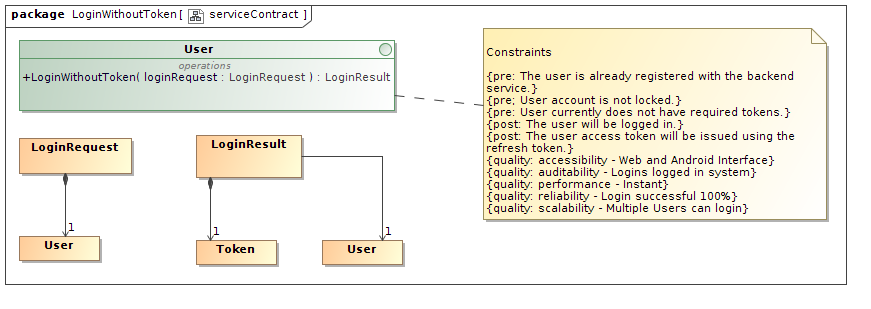
\includegraphics[scale=0.5]{loginWithoutToken}
				\caption{Login without Token Service Contract}
			\end{figure}
	\end{itemize}
	
\subsubsection{User Login - User holds access and refresh tokens}
	\begin{itemize}
		\item Description\\
		This use case will be used by the REST clients, specifically the Android app, to achieve safe long term login without storing user credentials on device. 
		\item Pre-Conditions
			\begin{enumerate}
				\item The user is already registered with the back-end service.
				\item User account is not locked.
				\item User currently has access and refresh tokens.
			\end{enumerate}
		\item Post-Conditions
			\begin{enumerate}
				\item The user will be logged in.
				\item The user access token will be updated using the refresh token.
			\end{enumerate}
		\item Service Contract
			\begin{figure}[H]
				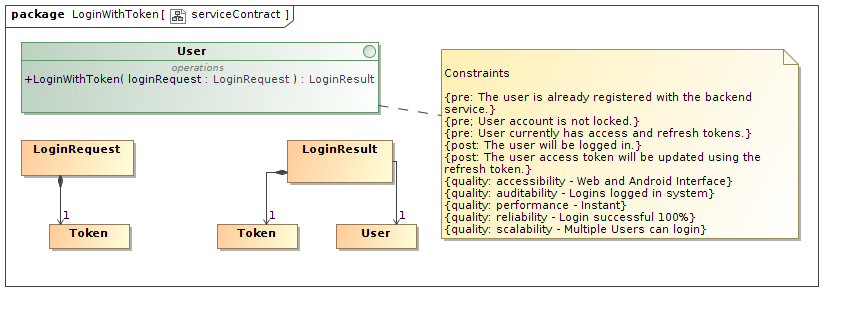
\includegraphics[scale=0.5]{loginWithToken}
				\caption{Login with Token Service Contract}
			\end{figure}
	\end{itemize}




\subsubsection{Log Out User}
	\begin{itemize}
		\item Description\\
			This use case will be used by the REST clients, specifically the web client and Android app, to log a user out of the system
		\item Pre-Conditions
			\begin{enumerate}
				\item The user is currently logged into the system
			\end{enumerate}
		\item Post-Conditions
			\begin{enumerate}
				\item The user will be logged out of the system
						
			\end{enumerate}
		\item Service Contract
			\begin{figure}[H]
				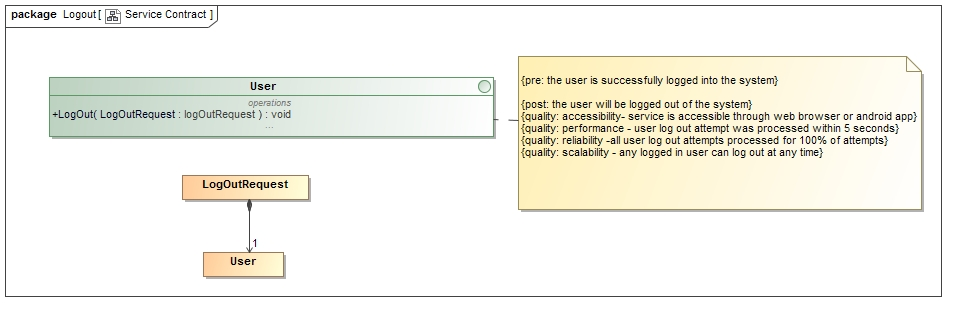
\includegraphics[scale=0.5]{Log_Out}
				\caption{Log the User out of the System}
			\end{figure}
	\end{itemize}

\subsubsection{Register User}
	\begin{itemize}
		\item Description\\
			This use case will be used by the REST clients, specifically the web client and Android app, to Create a user of the system
		\item Pre-Conditions
			\begin{enumerate}
				\item The user does not exist in the system
				\item All required details have been provided
				\item All details are valid
			\end{enumerate}
		\item Post-Conditions
			\begin{enumerate}
				\item The user will be created in the database
						
			\end{enumerate}
		\item Service Contract
			\begin{figure}[H]
				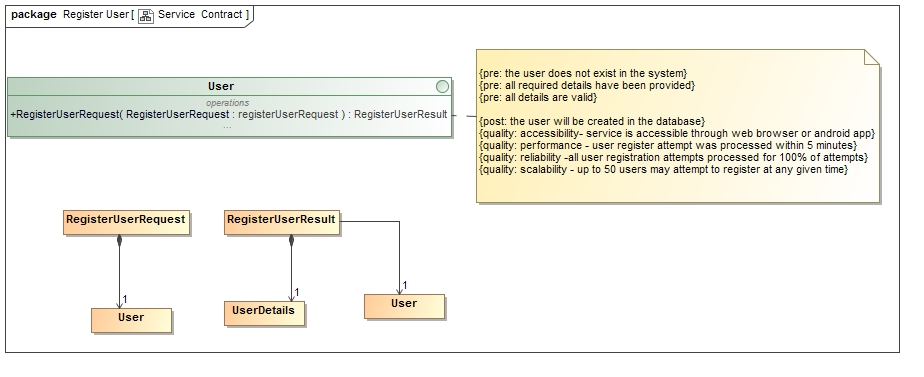
\includegraphics[scale=0.5]{Register_User}
				\caption{Register a User in the System}
			\end{figure}
	\end{itemize}
\subsubsection{View/Edit User}
	\begin{itemize}
		\item Description\\
			This use case will be used by the REST clients, specifically the web client and Android app, to View and Edit the currently logged in User
		\item Pre-Conditions
			\begin{enumerate}
				\item The user is succesfully logged in to the system
				\item Editted details are valid
			\end{enumerate}
		\item Post-Conditions
			\begin{enumerate}
				\item The user details will be editted
				\item All papers that the user is an author of should be displayed 
				\item User page will be displayed
						
			\end{enumerate}
		\item Service Contract
				\begin{figure}[H]
				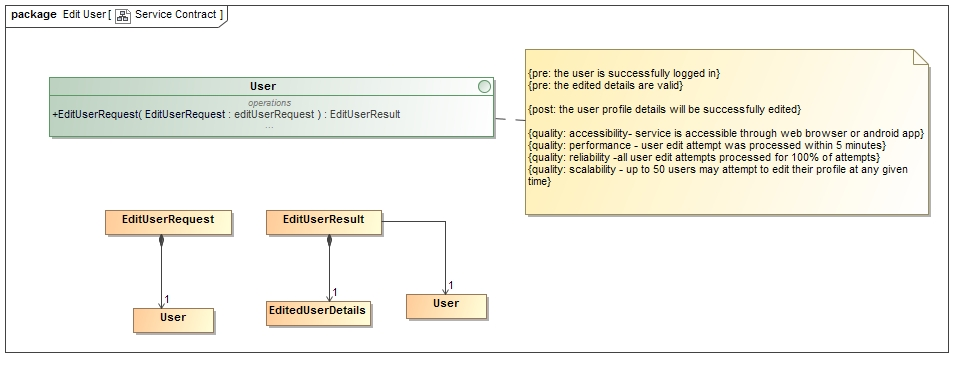
\includegraphics[scale=0.5]{Edit_User}
				\caption{Edit a User Profile in the System}	
				\end{figure}
	\end{itemize}

\subsubsection{Create Paper}
	\begin{itemize}
		\item Description\\
			This use case will be used by the REST clients, specifically the web client and Android app, to Create a Research Paper
		\item Pre-Conditions
			\begin{enumerate}
				\item The user is succesfully logged in to the system
				\item Paper details are filled in and valid
				\item The user must belong to a research group
			\end{enumerate}
		\item Post-Conditions
			\begin{enumerate}
				\item Paper succesfully created

						
			\end{enumerate}
		\item Service Contract
			\begin{figure}[H]
				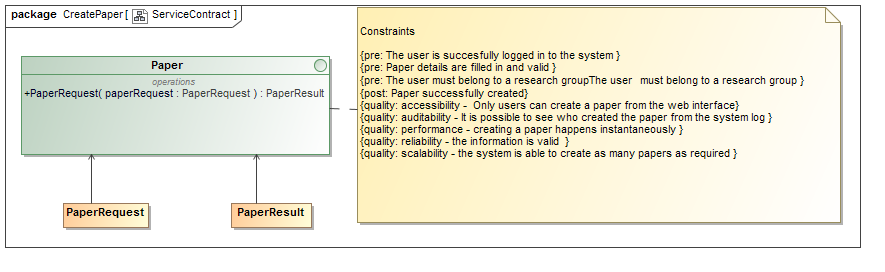
\includegraphics[scale=0.5]{CreatePaperServiceContract}
				\caption{Create Paper Service Contract}
			\end{figure}



	\end{itemize}

\subsubsection{Edit Paper}
	\begin{itemize}
		\item Description\\
			This use case will be used by the REST clients, specifically the web client and Android app, to Edit a Research Paper
		\item Pre-Conditions
			\begin{enumerate}
				\item The user is successfully logged in to the system
				\item The user is an Author of the Paper
				\item The user is an HOD or a Research Group Leader for the Group of the Paper
				\item The new details are valid
			\end{enumerate}
		\item Post-Conditions
			\begin{enumerate}
				\item The papers details will be edited
				\item The paper details will be displayed
						
			\end{enumerate}
		\item Service Contract
			\begin{figure}[H]
				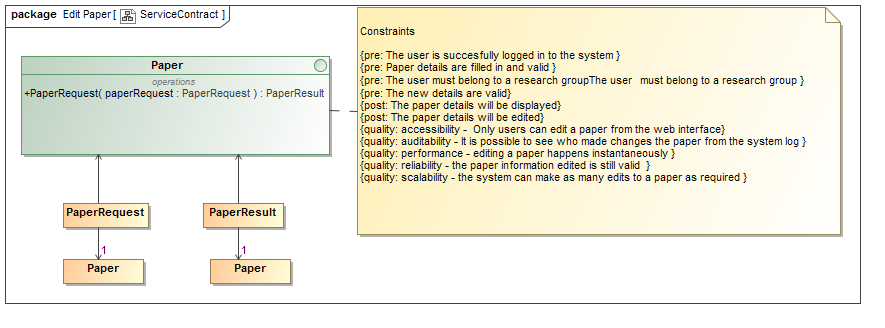
\includegraphics[scale=0.5]{EditPaperServiceContract}
				\caption{Edit Paper Service Contract}
			\end{figure}



	\end{itemize}

\subsubsection{View Paper}
	\begin{itemize}
		\item Description\\
			This use case will be used by the REST clients, specifically the web client and Android app, to View a Research Paper
		\item Pre-Conditions
			\begin{enumerate}
				\item The user is successfully logged in to the system
				\item The user is an Author of the Paper
				\item The user is an HOD or a Research Group Leader for the Group of the Paper
			\end{enumerate}
		\item Post-Conditions
			\begin{enumerate}
				\item The paper details will be displayed
						
			\end{enumerate}
		\item Service Contract
			\begin{figure}[H]
				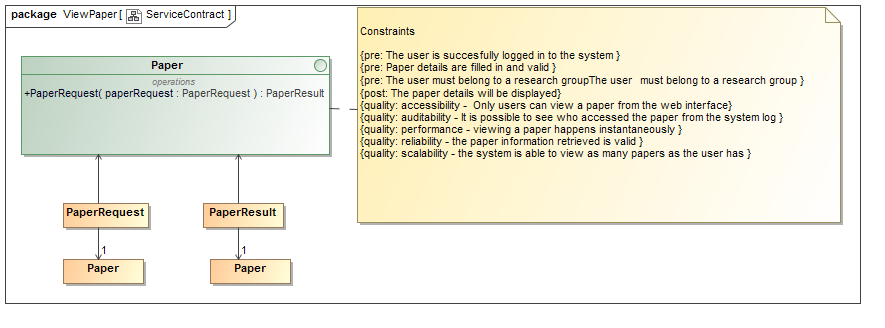
\includegraphics[scale=0.5]{ViewPaperServiceContract}
				\caption{View Paper Service Contract}
			\end{figure}

	\end{itemize}

\subsubsection{Create Author}
	\begin{itemize}
		\item Description\\
			This use case will be used by the REST clients, specifically the web client and Android app, to Create Authors
		\item Pre-Conditions
			\begin{enumerate}
				\item The user is successfully logged in to the system
				\item The details for the Author are valid
				\item The author must not previously exist in the system 
			\end{enumerate}
		\item Post-Conditions
			\begin{enumerate}
				\item The Author is successfully created	
			\end{enumerate}
		\item Service Contract
	\end{itemize}

\subsubsection{View/Edit Author}
	\begin{itemize}
		\item Description\\
			This use case will be used by the REST clients, specifically the web client and Android app, to View and Edit an Author
		\item Pre-Conditions
			\begin{enumerate}
				\item The user is successfully logged in to the system
				\item The new details are valid
			\end{enumerate}
		\item Post-Conditions
			\begin{enumerate}
				\item The Authors details will be edited
				\item The Authors details will be displayed
						
			\end{enumerate}
		\item Service Contract
	\end{itemize}


\subsubsection{Add/Remove Author to Research Paper}
	\begin{itemize}
		\item Description\\
			This use case will be used by the REST clients, specifically the web client and Android app, to Add and Remove Authors of a Research Paper
		\item Pre-Conditions
			\begin{enumerate}
				\item The user is successfully logged in to the system
				\item The user is an Author of the Paper
				\item The user is an HOD or a Research Group Leader for the Group of the Paper
				\item The new details are valid
			\end{enumerate}
		\item Post-Conditions
			\begin{enumerate}
				\item The Papers Authors have changed successfully
						
			\end{enumerate}
		\item Service Contract
			\begin{figure}[H]
				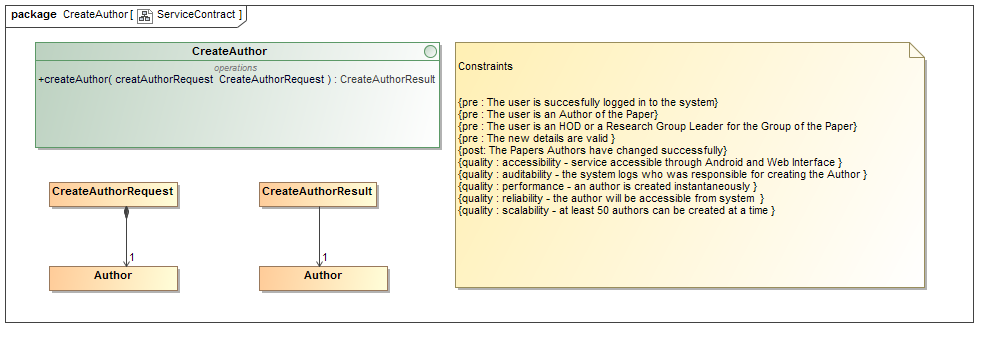
\includegraphics[scale=0.5]{CreateAuthorServiceContract}
				\caption{Create Author Service Contract}
			\end{figure}



	\end{itemize}

\subsubsection{Create Research Group}
	\begin{itemize}
		\item Description\\
			This use case will be used by the REST clients, specifically the web client and Android app, to Create a Research Group
		\item Pre-Conditions
			\begin{enumerate}
				\item The user is successfully logged in to the system
				\item The user is an HOD or a Research Group Leader for the Group of the Paper
			\end{enumerate}
		\item Post-Conditions
			\begin{enumerate}
				\item The Research Group is successfully added
						
			\end{enumerate}
		\item Service Contract
			\begin{figure}[H]
				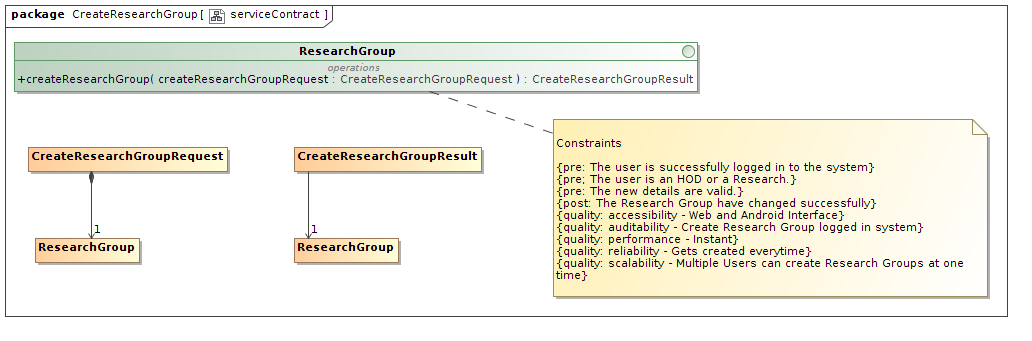
\includegraphics[scale=0.5]{createResearchGroup}
				\caption{Create Research Group Service Contract}
			\end{figure}
	\end{itemize}

\subsubsection{View/Edit Research Groups}
	\begin{itemize}
		\item Description\\
			This use case will be used by the REST clients, specifically the web client and Android app, to View/Edit a Research Group
		\item Pre-Conditions
			\begin{enumerate}
				\item The user is successfully logged in to the system
				\item The user is an HOD or a Research Group Leader for the Group of the Paper
				\item The new details are valid
			\end{enumerate}
		\item Post-Conditions
			\begin{enumerate}
				\item The Research Group have changed successfully
						
			\end{enumerate}
		\item Service Contract
			\begin{figure}[H]
				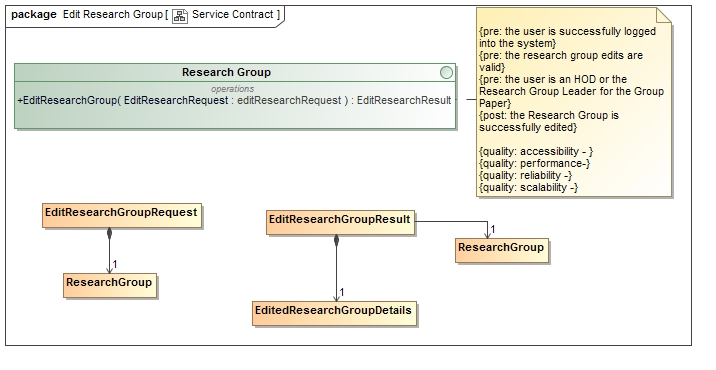
\includegraphics[scale=0.5]{Edit_Research_Group.jpg}
				\caption{Edit a Research Group's data in the System}
			\end{figure}
	\end{itemize}

\subsubsection{Add/Remove Users to Research Groups}
	\begin{itemize}
		\item Description\\
			This use case will be used by the REST clients, specifically the web client and Android app, to Add/Remove Users to a  Research Group
		\item Pre-Conditions
			\begin{enumerate}
				\item The user is successfully logged in to the system
				\item The user is an HOD or a Research Group Leader for the Group of the Paper
				\item The user is valid
			\end{enumerate}
		\item Post-Conditions
			\begin{enumerate}
				\item The User is successfully added to a Research Group
						
			\end{enumerate}
		\item Service Contract
	\end{itemize}

\subsubsection{Import Historical Paper}
	\begin{itemize}
		\item Description\\
			This use case will be used by the REST clients, specifically the web client and Android app, to Import a Historical Paper
		\item Pre-Conditions
			\begin{enumerate}
				\item The user is succesfully logged in to the system
				\item The paper details are correct
			\end{enumerate}
		\item Post-Conditions
			\begin{enumerate}
				\item The Historical Paper is sucessfully added
						
			\end{enumerate}
		\item Service Contract
	\end{itemize}

\subsubsection{Generate Bibliography}
	\begin{itemize}
		\item Description\\
			This use case will be used by the REST clients, specifically the web client and Android app, to Generate a Bibliography for a User
		\item Pre-Conditions
			\begin{enumerate}
				\item The user is succesfully logged in to the system
			\end{enumerate}
		\item Post-Conditions
			\begin{enumerate}
				\item Bibliography sucessfully generated
						
			\end{enumerate}
		\item Service Contract
			\begin{figure}[H]
				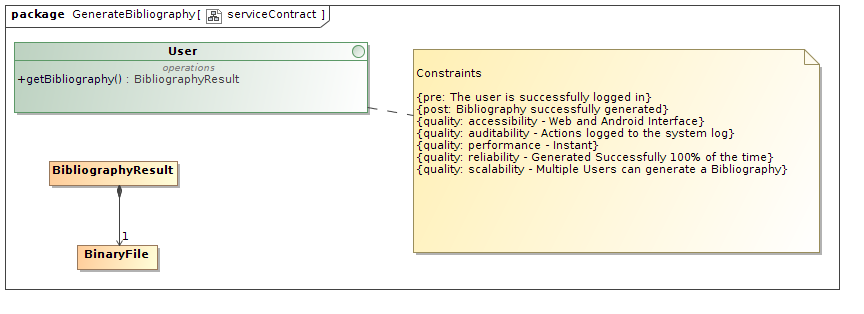
\includegraphics[scale=0.5]{generateBibliography}
				\caption{Generate Bibliography Service Contract}
			\end{figure}
	\end{itemize}


\subsubsection{Create Venue}
	\begin{itemize}
		\item Description\\
			This use case will be used by the REST clients, specifically the web client and Android app, to Create a Venue
		\item Pre-Conditions
			\begin{enumerate}
				\item The user is succesfully logged in to the system
				\item Venue details are valid
			\end{enumerate}
		\item Post-Conditions
			\begin{enumerate}
				\item The Venue is succesfully ediited
						
			\end{enumerate}
		\item Service Contract
	\end{itemize}

\subsubsection{View/Edit Venue}
	\begin{itemize}
		\item Description\\
			This use case will be used by the REST clients, specifically the web client and Android app, to View/Edit a Venue
		\item Pre-Conditions
			\begin{enumerate}
				\item The user is succesfully logged in to the system
				\item The new details are valid
			\end{enumerate}
		\item Post-Conditions
			\begin{enumerate}
				\item The Venue is succesfully ediited
						
			\end{enumerate}
		\item Service Contract
	\end{itemize}


\subsubsection{View Log}
	\begin{itemize}
		\item Description\\
			This use case will be used by the REST clients, specifically the web client and Android app, to view a system log
		\item Pre-Conditions
			\begin{enumerate}
				\item The user is succesfully logged in to the system
				\item The user must be a Super User
			\end{enumerate}
		\item Post-Conditions
			\begin{enumerate}
				\item The system log will be displayed
				
						
			\end{enumerate}
		\item Service Contract
	\end{itemize}



\subsection{Required functionality}

\subsubsection{Edit Research Group}
	\begin{figure}[h]
		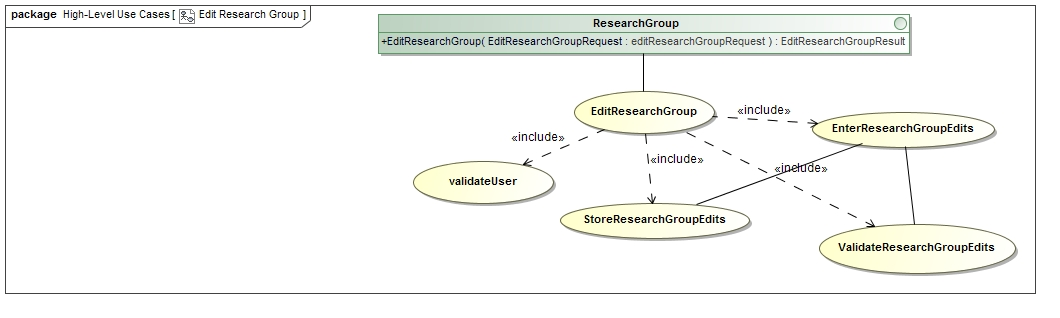
\includegraphics[scale=0.5]{UseEditResearchGroup}
	\caption{Use Case for Edit Research Group}
	\end{figure}
	
\subsubsection{Edit User}
	\begin{figure}[h]
		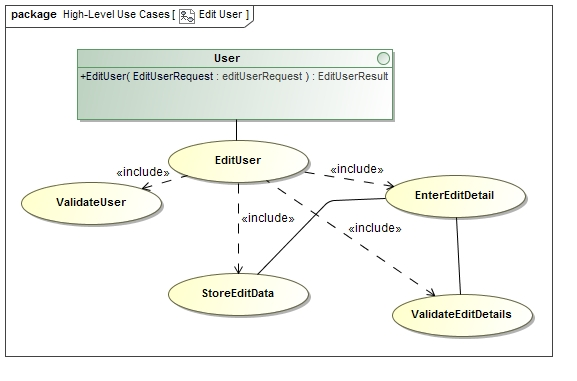
\includegraphics[scale=0.5]{UseEditUser}
	\caption{Use Case for Edit User}
	\end{figure}
		
\subsubsection{View User}
	\begin{figure}[h]
		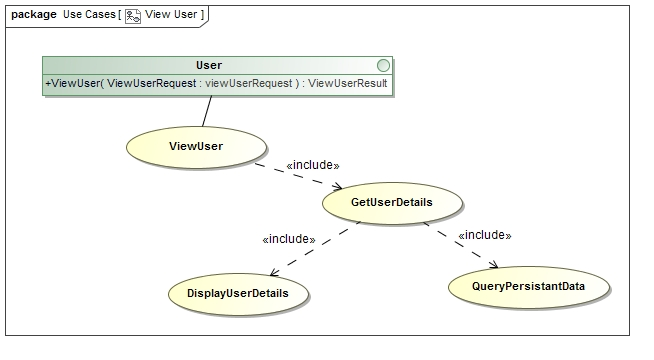
\includegraphics[scale=0.5]{UseViewUser}
	\caption{Use Case for View User}
	\end{figure}
		
\subsubsection{User Log Out}
	\begin{figure}[h]
		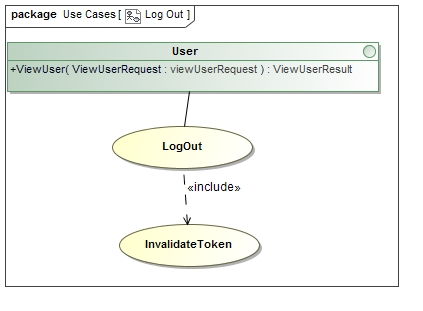
\includegraphics[scale=0.5]{UseLogOut}
	\caption{Use Case for User Log Out}
	\end{figure}	
\subsubsection{Register User}
	\begin{figure}[h]
		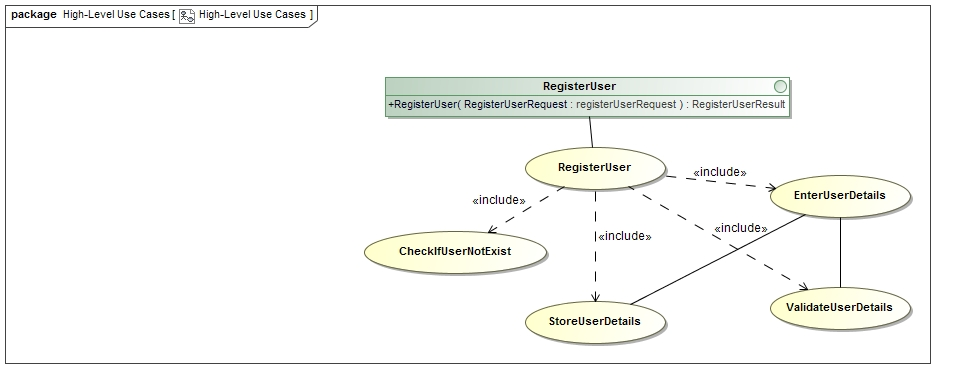
\includegraphics[scale=0.5]{UseRegisterUser}
	\caption{Use Case for Register User}
	\end{figure}

\subsection{Process specifications}
\subsubsection{Edit Research}
	\begin{figure}[h]
	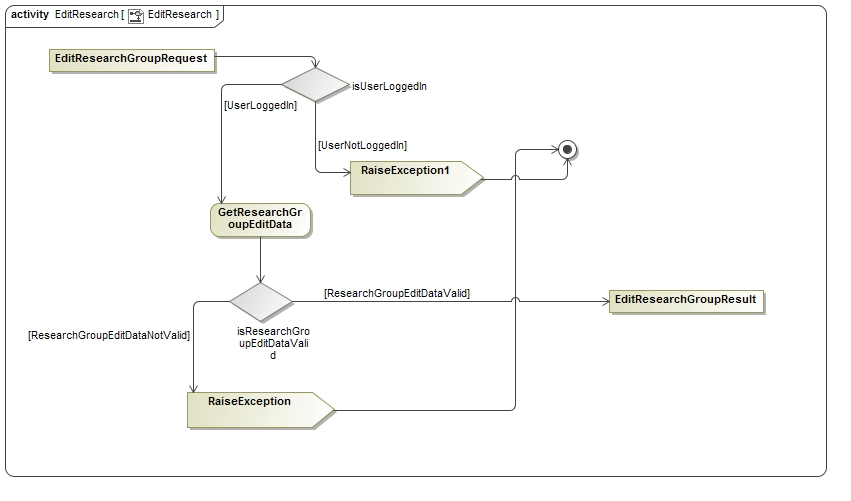
\includegraphics[scale=0.5]{ActEditResearch}
	\caption{Process Specification for Edit Research}
	\end{figure}
	
\subsubsection{Edit User}
	\begin{figure}[h]
	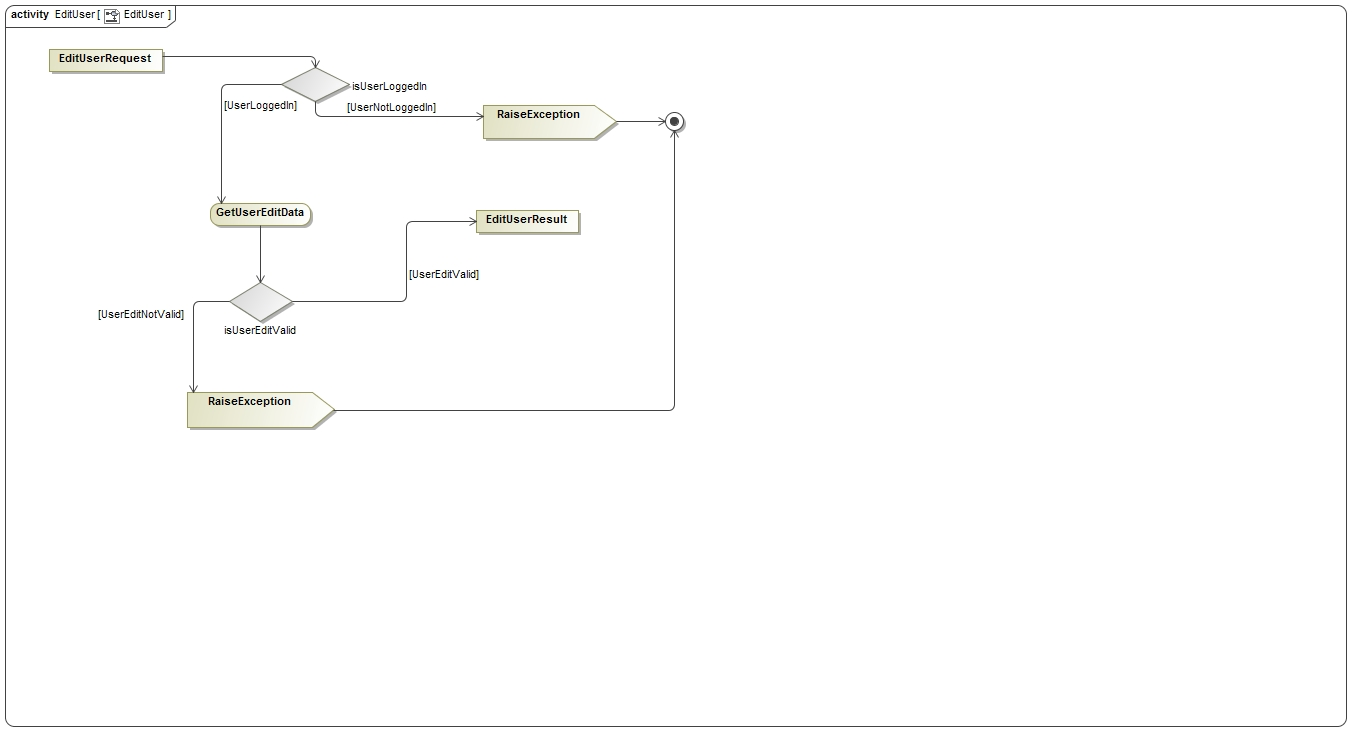
\includegraphics[scale=0.5]{ActEditUser}
	\caption{Process Specification for Edit User}
	\end{figure}
		
\subsubsection{Log Out}
	\begin{figure}[h]
	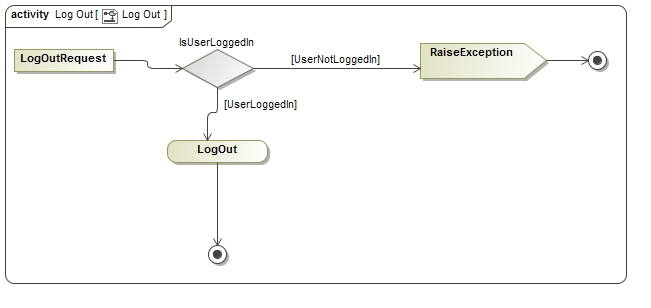
\includegraphics[scale=0.5]{ActLogOut}
	\caption{Process Specification for Log Out}
	\end{figure}
		
\subsubsection{Register User}
	\begin{figure}[h]
	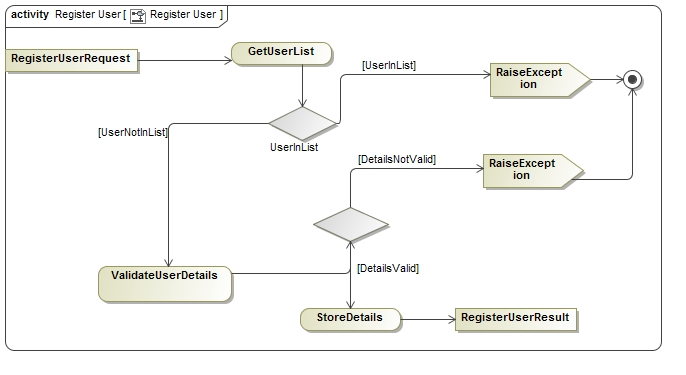
\includegraphics[scale=0.5]{ActRegisterUser}
	\caption{Process Specification for Register User}
	\end{figure}
		
\subsubsection{View User}
	\begin{figure}[h]
	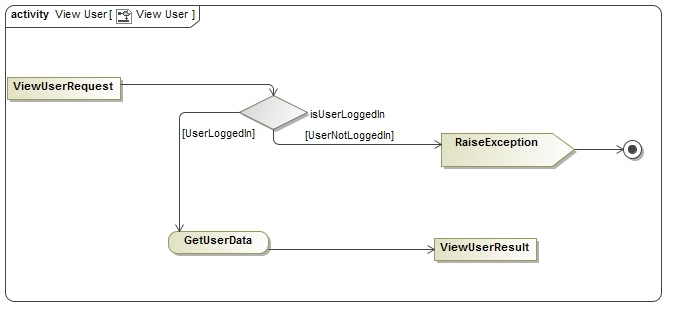
\includegraphics[scale=0.5]{ActViewUser}
	\caption{Process Specification for View User}
	\end{figure}	
	
\subsection{Domain Model}

\section{Open Issues}
\subsection {GitHub Repository}
Team Echo Repository: \url{https://github.com/andrewbroekman/echo}

This repository contains:
\begin{enumerate}
\item All work done by team members.
\item \href{https://github.com/andrewbroekman/echo/blob/master/CONTRIBUTORS.md}{CONTRIBUTORS.md} file outlining which members where involved in which phases of the project.
\end{enumerate}

\begin{appendices}
\newpage
\section{Data Dictionary}
\begin{tabu} to \textwidth { | X[l] | X[l] | }
	\hline
		\textbf{Term}		& \textbf{Definition}	\\ \hline \hline
		Android			&  A Linux based operating system developed by Google Inc. and the Open Handset Alliance for smart phones, tablets, and other mobile computing devices. Android applications are developed in Java. \\ \hline
		HTTP			& HyperText Transfer Protocol, standardised by RFCs 7230-7237 \\ \hline
		ISO				& International Organization for Standardization \\ \hline
		MVC				& Model-View-Controller \\ \hline
		OAuth			& An open standard for authorization, using an access token approach, allowing resource owners to authorize third-party clients to access protected user resources on a resource server, without the client providing their credentials to the third-party in question. \\ \hline
		RDBMS			& Relational Database Management System \\ \hline
		SPA				& Single Page Application \\ \hline
		SQL				& Structured Query Language is a programming language, standardised by ISO for managing data in RDBMS. Actions allow for the creation, reading/retrieving, updating and deletion of data in the management system. \\ \hline
	\hline
\end{tabu}

\end{appendices}

\newpage
\clearpage
\addcontentsline{toc}{section}{References}
\printbibliography



\end{document}
